% \textbf{Title: Filtering 3}

Consider the first 100 components of the Fourier series of a square wave. For reference, \(b_{n} = \frac{4}{\pi\text{n}}\) for odd \(n\) and zero for even \(n\), where \(b_n\) are the Fourier sine series coefficients. This signal is sent through an ideal filter, which outputs this signal.

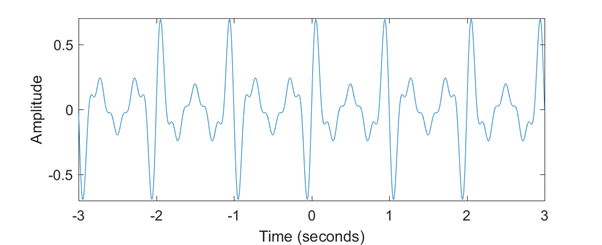
\includegraphics[width=5in,height=2in]{../../Images/FilteringQ3.png}

What kind of filter could this be?\\

a. A high-pass filter.

*b. A band-pass filter.

c. A low-pass filter.

d. A band-stop filter.

e. I do not know.\\
